\documentclass[a4paper,twoside,10pt]{report}
\usepackage[english]{babel}
\usepackage[utf8]{inputenc}
\usepackage{graphicx}
\usepackage{url}
\usepackage[export]{adjustbox}
\usepackage{indentfirst}
% pdflatex

% redefinição das margens das páginas
\setlength{\textheight}{24.00cm}
\setlength{\textwidth}{15.50cm}
\setlength{\topmargin}{0.35cm}
\setlength{\headheight}{0cm}
\setlength{\headsep}{0cm}
\setlength{\oddsidemargin}{0.25cm}
\setlength{\evensidemargin}{0.25cm}
\setlength{\parskip}{1em}

\begin{document}

\begin{figure}[t]
\resizebox{60mm}{!}{
\includegraphics[left]{logoISEL.png}}
\end{figure}

\title{\huge\textbf{Lean Dashboard}}

\author{
\begin{tabular}{c}
José Pedro Jesus, n.º 44805\\
Hugo Manuel Jacinto Pinheiro, n.º 44886\\
Tomás Simão Mendes dos Santos, n.º 45363\\
\end{tabular}
}

\date{
\begin{tabular}{ll}
  {\textbf{Supervisors:}} & João Pereira, e-mail: joao.pereira@inetum.world, Inetum \\
                 & Filipe Freitas, e-mail: ffreitas@cc.isel.ipl.pt\\
\end{tabular}\\
\vspace{80mm}
\textbf{June 14th 2021}}

\maketitle

\title{\huge\textbf{Abstract}}

The amount of information necessary to develop an application nowadays is a lot to keep track of. Suppose you're a project manager and you want to keep track of the information of your project as well as show it to your team but it is scattered across different platforms.

Data ranging from test results to the current sprints can all be puzzle pieces of a much bigger picture and accessing the various platforms only to view this information can be tiring and complicated.This project's goal is to simplify a team's life, by developing an application that allows a project manager to control and show the team members the necessary information for their project.

This application will make use of a single page application, a web server(Web API), as well as a no-SQL database and an ETL procedure used to extract and transform the information from the various data sources.


\textbf{Keywords:} Information Aggregation, ETL, Project Managing, Project Information, Team Management, Single Page Application, Web API, no-SQL Database


\newpage
\tableofcontents{}
\newpage

\chapter{Introduction}

Nowadays, within a company, it is even more important to have an organized and cooperative team with knowledge of all the steps and goals that need to be worked on for the various projects they are currently participating in.
Each member of the team must keep track of high amounts of information and since it is not uncommon that when working on a project a couple of platforms are used to keep track and share work done by the various members, useful information can be scattered on a vast amount of platforms, and sometimes even inside a single platform.
The information relative to a project can be obtained from different sources and it is all aggregated in one place, readily available to be displayed to a work team to better guide a certain project's development.

The Lean Dashboard Project will be developed to help the company's workers keeping track of all the possible tasks for their projects, gathering all the information needed for the various activities from the many sources that are necessary, presenting it on an easy to read and reactive web application.
The project at hands will be developed in partnership with Inetum\cite{INETUM} and will centre around the development of a responsive web application capable of running on a multitude of devices, ranging from smartphones to desktop computers to large screens such as TV’s. This web application will display to a work team of a company all the information regarding various projects being worked on. 
The information being displayed will show the team what needs to be addressed in the project at hands, such as milestones, bugs, and current errors in the project.

\section{Report Organization}
In this report, we will explain the early drafts of the implemented solution to the problem at hands, as well as provide a more in-depth analysis of the architecture and technology choices.

In the Functionalities chapter, we will expose which features from the project are currently implemented and working, as well as the ones that are yet to be implemented. Additionally, we also showcase a couple of aspects regarding planning and research.

Next up, in the Architecture chapter, we will discuss aspects such as the implementation of the software being developed, decisions made by us and how certain problems were solved.

Furthermore, we dedicate a chapter to the research done in regards to User Experience for our application where we will display some of the steps we took in preparing our client application in terms of User Experience.

Finally, the Client Application chapter. Here, we explain the reason for the chosen development platform and display some of the pages that are already made.  



\chapter{Functionalities}
The functionalities section is destined to list and describe the functionalities that the final application will provide the user with.

In this section, information such as what is already implemented within the application, the research and planning that was made for the project and, the functionalities that will still be added to the project can be found in more detail.

All of this information will be updated in future reports as we continue to improve the project.


The solution will be a responsive mobile-first web application that will allow to consult and aggregate the information of various platforms. Inside a project, a manager will be able to add various dashboards that will then have the desired widgets. The widgets are the structures that hold and show the desired information regarding issues, tests, and sprints from platforms such as Jira\cite{JIRA}, Squash\cite{SQUASH} and Azure\cite{AZURE}. A manager will then be able to add various users to its project so that those users can consult all the dashboards with the relevant information in each widget.
\section{Implemented functionalities}
By the time of the delivery of this report, this are the features implemented:
 
\begin{itemize}
     \item Retrieving the data from the multiple APIs. As of right now, we can access the three supported APIs to obtain the relevant information
    
     \item Authentication of local users using the Authization Module. With the help of the module, we can now create new users, log in and logout out of users of local accounts.
    
     \item In addition to users, we also support roles for the given users: Superuser, Manager and Collaborator. Further on we will address these Role-based access control\cite{RBAC} (RBAC) roles and permissions
    
     \item Back-office implementation was started. With this, managers can now do actions such as add new members to a project, remove current project members as well as give certain users roles

     \item Creating new projects. Authorized users can add new projects to the platform and manage them

     \item Creating various Dashboards inside an existing project. After creating a project, it is also possible to include new dashboards in said project

     \item Transforming the retrieved data in a widget format. The retrieved data is not yet in the desired format and needs to be adapted (we will cover the formatting of widgets later on in this report)

     \item Creating a widget and adding it to an existing dashboard with the use of existing templates, that aid the user by showing them the type of existing widgets.

     \item Automatically updating widgets with the use of a scheduler. Users can set a period to refresh existing widgets, making sure the most up to date information is being displayed. The process and technology chosen for the scheduler will be explained in the back end portion of this report

     \item Setting the credentials for all the platforms. When creating a widget, a user can set up the desired credentials, to choose the data source for a specific widget
\end{itemize}

\section{Research and planning}
In this section, we display the set of aspects, that despite technically not being functionalities, are essential aspects for the development of this project:

\begin{itemize}
    \item Digital prototype of the User Experience. The Digital prototype developed allowed us to conduct a series of usability tests (that are still ongoing). Details about these tests will be discussed further ahead in the report
    \item Red routes diagram. This diagram is part of the Experience research further developed ahead.
    \item Information architecture\cite{INFOARCH}. A diagram that displays the existing paths/flows of the client application
    \item Study of the React\cite{REACT} technology for the development of the client application
\end{itemize}

\section{Functionalities to be added}
\begin{itemize}
    \item Finishing management of projects by the back-office manager. Add functionalities such as deleting users and changing usernames
    \item Full authentication and authorization
    \item Revisiting the structure of widgets. As more widgets are added to the application, re-analyzing the structure of widgets is an important step
    \item Finishing the client application with the React technology 
\end{itemize}

\chapter{Architecture}
This chapter is dedicated to cover topics like the software's architecture, the data model and the principles under which the application is being developed. 

It contains information on how the application works and how its various modules and components interact with each other, as well as the structure of the necessary information being stored in the database and the application's authentication and authorization flow.
\section{Architecture Principles}
The software solution being developed in the Lean Dashboard is divided into three main components: the ETL\cite{ETLPROC}, the Lean Dashboard Server and the client application.
 
The ETL component, which stands for Extract, Transform and Load,  is responsible for obtaining the information from the various APIs and then transforming it to the desired format, widgets, and then proceeding to store them in a database. Both the topics of widgets and the storage solution being used will be addressed in this report in the Data model.
 
With the use of the ETL procedure in our application, we bring a couple of advantages to the way we interact with the data being displayed. Since having near-real-time information is enough, with the Extract component we can avoid making high amounts of requests to the various APIs and avoiding overload them.
 
Additionally, by adapting the extracted information (the Transform component) we can have a format of data that closely resembles the type and aspect of details we are trying the show to the user in each widget (we will also showcase the aspect of a widget in our application).Finally, with the information transformed to the desired format, when can then use a No-SQL database to store it and later decide how we will display it to the users 
 
The Lean Dashboard server ends up serving as a gatherer of information. Inside this server, we will have all of the various projects, created by users, and each one will have its dashboards. Dashboards will be used to group the various widgets, and the user is the one to choose which dashboards will contain which widgets (these being the same widgets that we're created by the Extract, Transform and Load procedure).
 
Lastly, we have the client application. The client application will be responsible for showing the user all of its projects. Users (if they are given these permissions) will be able to consult but also edit projects and dashboards. The main goal will be checking on the widgets inside a certain dashboard since those are the objects that contain the information being retrieved and transformed by the ETL.

\section{Software Architecture}
\begin{figure}[h!]
\center
    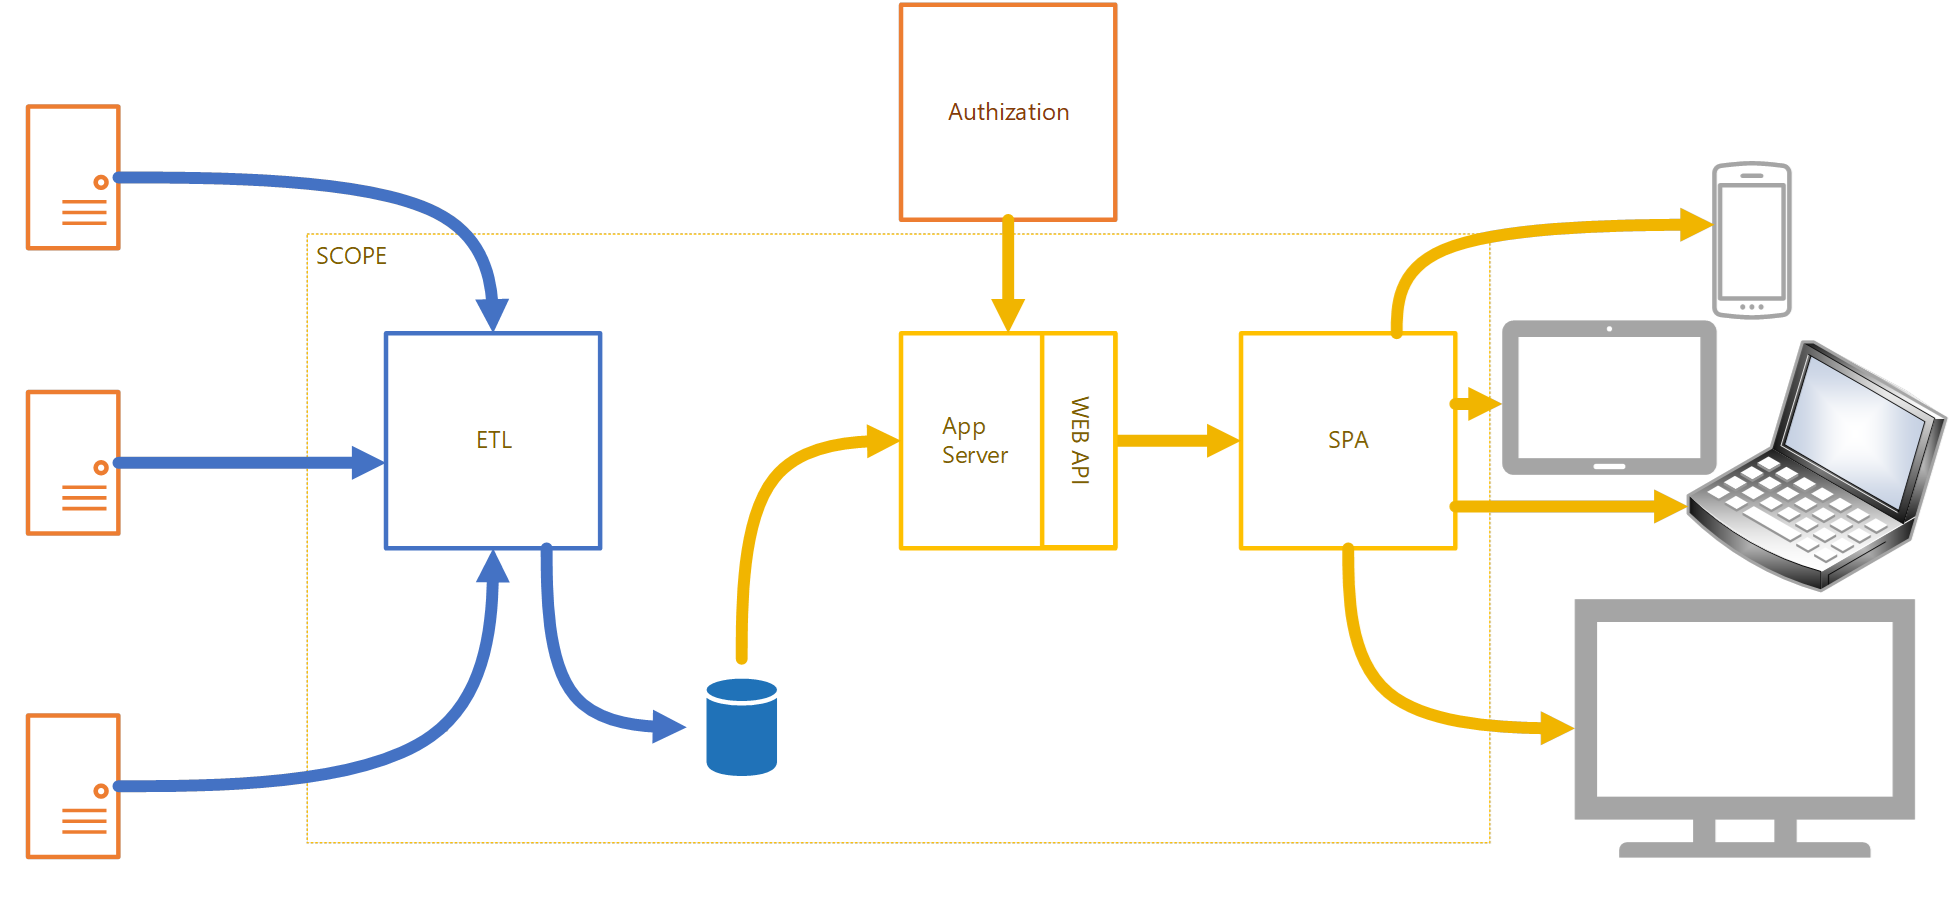
\includegraphics[width=\textwidth]{lean-dashboard-software-architecture.png}
    \caption{Lean Dashboard's Software Architecture and component interactions}
\end{figure}
On Figure 3.1 it is depicted the various components of our application interacting with each other.

The rightmost part represents the information sources. These sources provide its users with an Application Programming Interface (API), this API will be used by the  ETL to obtain solely the needed information.

This information can take different forms. The data objects received from the APIs will differ in terms of structure and information, for example, a project is different from an issue. This means it is crucial to implement an optimized Extract module within the ETL component of our application.

After extracting this information, the ETL will send it towards its respective Transformation module, where it will be treated and converted into a new data object with the necessary fields to represent it visually later.

The Load module of the ETL will grab this newly created Widget object and load it on a database.

The ETL procedure is constantly running and updating the existing widgets on the database, according to the widget's time settings that will be presented in this document.

In the middle of the scheme is the core of the application, the Web Server, and its API.

The Web Server is responsible for processing the requests that will be sent by the Single Page Application (SPA), as well as managing the NoSQL database running on ElasticSearch\cite{ES}.

It interacts with an authorization and authentication module, the Authization module, to manage the users and their roles within the application.

The API supports a varied range of operations that can be called by the user to manipulate the information inside the database. It presents the user with methods to obtain, create, update, and delete the information in the database.

Lastly on the rightmost side of the diagram, there is the SPA, the component that will be accessed by the application user on their preferred device. To provide the user with the best experience, this SPA will be developed as a mobile-first, responsive web application capable of supporting different types of display screens, starting from the smartphone up to the bigger ones like a regular desktop computer or a TV screen.
\newpage
\section{Scheme of the back-end}
\begin{figure}[h!]
\center
    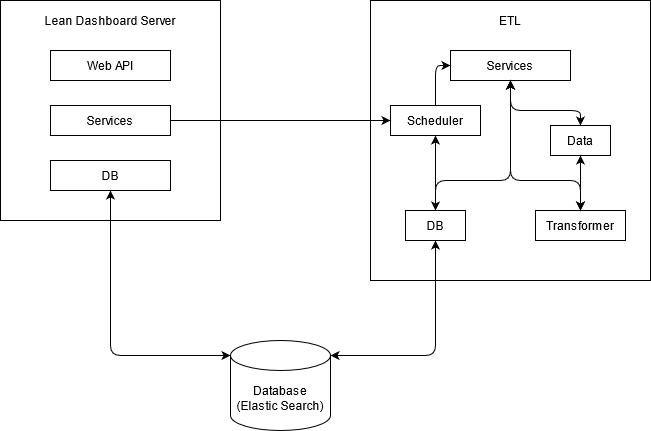
\includegraphics[width=\textwidth]{arquitetura software.png}
    \caption{Back-end structure and modules interactions}
\end{figure}
Figure 3.2 depicts the application's back-end and the information flow between its main components. On the left, we have the Lean Dashboard Server and on the right the ETL Procedure, the two key components of the application's back-end.

These two components interact with one another so that the ETL knows what sort of information it should obtain.

The Lean Dashboard Server is composed of 3 Node.JS\cite{NODE} modules:
\begin{itemize}
  \item The Web API module is responsible for catching the requests sent to the API, filtering the parameters and body fields, and sending them to the Services module.
  \item The services module will process every request the Web API receives and forms a function call to the Database(DB) module. If the request consists of modifying or creating a Widget object it will make a call towards the Scheduler module in the ETL.
  \item The DB module is responsible to access and modify the ElasticSearch based database, containing all the necessary functions to create, obtain, delete and edit the database. It also verifies if the inputted parameters are valid within the context of the application, preventing the existence of duplicates or the association of members to a project who aren't registered in the application, for example.
\end{itemize}
\newpage
The ETL component, as we already mentioned, is responsible for accessing the various data sources and transforming them into a specific widget object.

It contains 5 Node.JS modules in its structure:
\begin{itemize}
  \item The Scheduler module, accessed by the lean-Services module, is responsible for scheduling the automatic ETL process that will update the created widgets according to the time settings a user provides. It accesses the DB module to retrieve the necessary information to execute the correct Services function.

The module is implemented using the node-cron\cite{NODECRON} module so that we can easily create and configure jobs to execute at a set time.
It contains 2 Map objects with distinct functionalities, the widgetMap is responsible for providing the scheduler with the necessary ETL-Services function to execute for the various widgets according to the function parameter contained within the widget's structure, and the widgetJobs associates a widgetId to its currently running job so that we can reconfigure them at a later date.
  \item The ETL-Services module acts as a coordinator for the ETL procedure, it obtains the necessary filtered data from the Data module and then gets the transformed information from the Transformer module.

After the process of obtaining information is complete it calls the DB module so that this information can be stored.
  \item The Data module's task is accessing the selected information sources, currently Azure, Jira, and Squash, and sending them to the Transformer module for some light filtering, returning the retrieved object with only the necessary information for its transformation.
  \item The Transformer module's job is to transform the data into the required information for the widget to be displayed. Currently, it transforms the data into widgets such as a Pie Chart, a Data Table, or a Gauge Chart.
  \item Finally, the DB module is responsible for updating the widget's information with the updated data obtained from the ETL procedure.
\end{itemize}

\newpage
\section{Data Model}
For the Data model and the storage of the information, we chose the No-SQL database Elastic Search.
 
To better facilitate the getting and storage of information, we divided each object into they're own index, as displayed in the following scheme:

\begin{figure}[h!]
    \center
    \resizebox{120mm}{!}{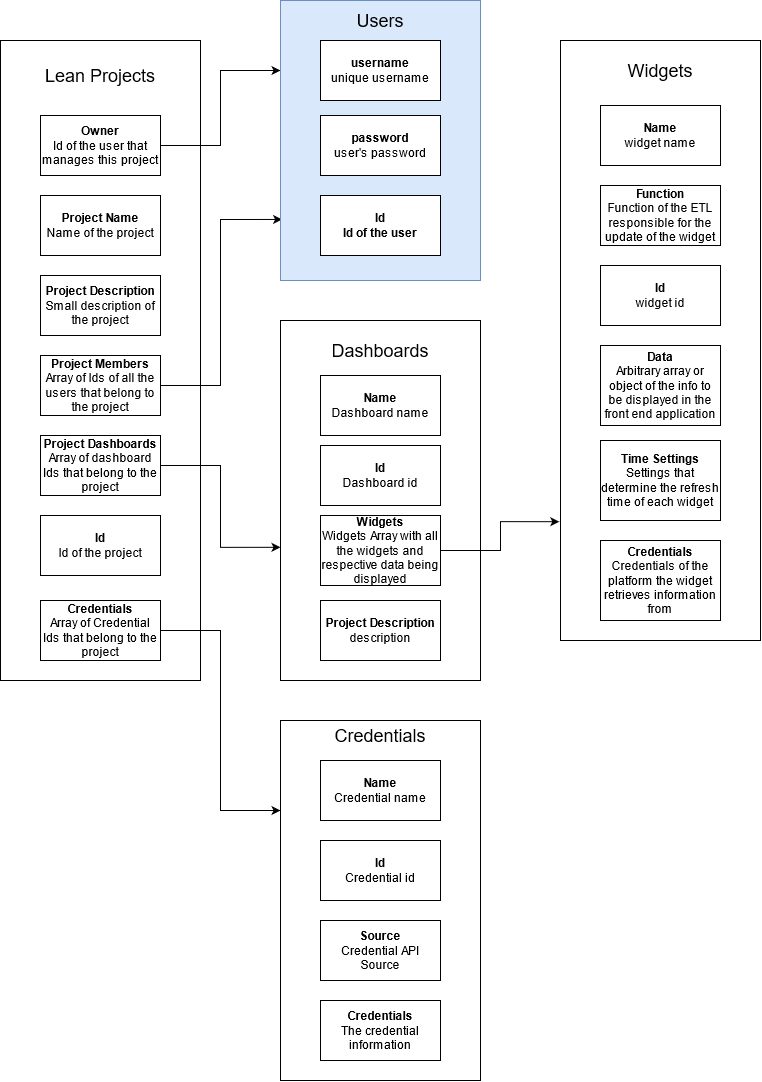
\includegraphics[width=\textwidth]{modelo de dados.png}}
    \caption{Database Data Model}
\end{figure}

Figure 3.3 depicts the application's data model and the object's structures. Each of these objects contains the necessary fields to store the needed information for the application. 
\newpage
Each object is detailed as the following:
\newline

\textbf{Lean Projects}

This is the index where all the Projects created with our application will be stored, acting as the main gatherer of information.

It has information over who created it (Owner), the Project's name, its description, and a unique identifier.

Each project can contain a varied number of members, dashboards, and credentials. 

This information is stored inside an Array of identifiers, these being Project Members for the members that are currently associated with the project, Project Dashboards for the dashboards, and Credentials for the credentials.

The members simply act as viewers of the information within the project, they can only access dashboards and view the information on the widgets.


\textbf{Users}

The users are highlighted in a different color on the scheme to better differentiate them from the data model since they aren't being stored in the database our application manages and are being stored in the Authization module's database.

Each user will have a username and a password so they can log in to our application, as well as a unique identifier within the database to be used by the array of members within the Lean Projects Objects.


\textbf{Dashboards}

The dashboards are where the widgets will be stored. They don't exist if there isn't at least an already existing Lean Project and will be presented as a web page with all the widgets within the dashboard being displayed.

The dashboard objects contain a name, an Array of Widget identifiers that are associated with the dashboard, a description, and a unique identifier within the database.


\textbf{Credentials}

The credentials consist of a specific object containing a name, a source (Azure, Jira, or Squash), and a credential object containing all the credentials themselves.

This credential object is structured as such for each of the information sources:

\begin{figure}[h!]
\center
    \resizebox{120mm}{!}{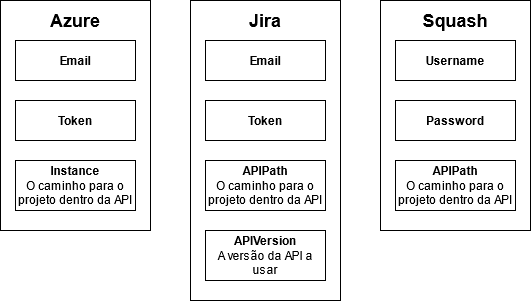
\includegraphics[width=\textwidth]{formato das credentials.png}}
\caption{Credentials and their structure for each data source}
\end{figure}

Each source requires a different form of credential so that the authentication on their web API is successful. These credentials are mandatory as the ETL procedure cannot access the specified information source's API without them.
\newline
According to figure 3.4:
\newline

Azure requires an email, a token, and an Instance field related to the project within the API.

Jira requires an email, a token, an APIPath for the project within the API, and an APIVersion that refers to the API version to be used.

Squash only requires a username, a password, and the APIPath.

\newpage

\textbf{Widgets}

The widgets are the result of the ETL procedure.

They are created by the user through the selection of a widget template that will serve as a widget with temporary data to be displayed.

Widgets are made out of several fields like a name, a function, a data object, the time settings for the ETL schedule, the required credentials, and a unique identifier.

The function field refers to which ETL function the scheduler needs to call to start the node job.

The time settings are an object that contains information related to the interval at which the ETL procedure is executed to update the widget. 

Each field of this object is structured in CronTab format and consists of:
\begin{itemize}
  \item seconds;
  \item minutes;
  \item hours;
  \item day of the month;
  \item month;
  \item day of the week;
\end{itemize}
The credentials are the credential object associated with the project.

Without them obtaining information is impossible, making it a required field when creating the widget.

The data object is where all the transformed ETL information will be stored. It is the main reason the application utilizes an ElasticSearch database, as the information contained within this object will vary from widget to widget, making it a hard task to store consistently within a relational database like PostgreSQL.


\newpage
\section{Authization module, Backoffice and Access control}
 To give our users authorization and authentication features we had to think of a way of letting users create accounts, have users with different roles inside the application and have different roles have their privileges. To give users that set of features, and as a request of Inetum, we utilized a Node module called Authization\cite{AUTHIZATION}. 

As a reference point, this module was a project developed last year by the ISEL students Tiago Matias, Diogo Leandro and João Barata of the LEIC programme as a final project of the Project and Seminar course, and was also developed in partnership with Inetum, and serves as a module that allows to set up an RBAC model with various roles, permissions and decide which roles should have access to what permissions. The module will also take care of aspects such as login, logout and the creation of users. Since the module requires a SQL Database for the storage of users, we had to use  PostgreSQL\cite{POSTGRESQL} to handle the storage of users, the created roles and permissions.

As for the RBAC model, it was requested that there were three types of users: a master user, with every kind of accesses and ultimate control (that includes access to every existing project, both seeing and editing them), a user that would be able to manage certain projects and create new ones and finally a user with only permission to see projects he is a part of.
With that said, we came up with an RBAC model with the roles Superuser, Manager and Collaborator, with the following accesses:
 

\begin{figure}[h!]
\center
    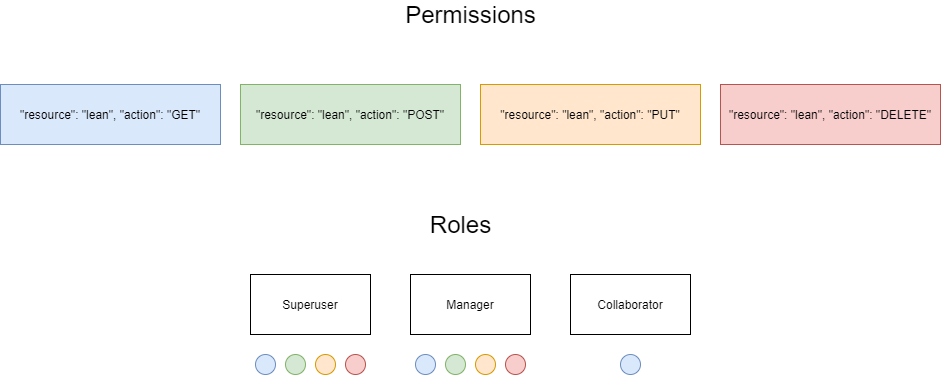
\includegraphics[width=\textwidth]{lean-rbac-model.png}
\caption{Application User Roles and their respective permissions}
\end{figure}
As said before, we defined three roles. The Superuser will have access to all of the defined permissions, being able to access and modify all projects,  without having to be a part of them. 
Below the Superuser, the Manager role will act in a similar way to the Superuser, but will only be able to modify projects that we're created by himself. Additionally, he will only be able to visualize projects (and the dashboards and widgets associated with the said project) if he is a member or instead, the creator of that project. A manager will be able to manage aspects of a project such as its name, description, containing dashboards and widgets, as well as all the members in it.
Finally, the role of Collaborator. Being the role with fewer permissions, users with this role will only be able to access projects they are members of.

\chapter{User Experience Research}
This section will cover our User Experience research and studies on how our application will be controlled.

Our research on every necessary item to develop an application that is easy and intuitive to use and will be presented here.

User Experience, commonly called UX, is the term used when referring to how users interact with a certain product. If we use an analogy, if we were to open a door, it is more about how the door handle is used than what shape or colour it has, or what material it is made from. 

UX is also greatly impacted by the context a product is being used and the type of users using said product. Inetum conducted a UX research using contextual interviews with potential users of Lean Dashboard in order to understand their real needs. After studying the observations, 2 Personas were created that focus on the needs of the real target. That list of personas would help us take into consideration how we would address the UX design of our early digital prototypes (which later reflect on the client application), by having various types of users with specific personalities, most wanted features and specific positions inside a company. 

Following that, we developed a digital prototype that would allow us to make a series of usability tests with real users. Those tests would allow us to better determine what needed to be addressed in our digital prototype and solve issues before any implementation was being done.

With that said, we believe the User Experience research done by the group is something that can greatly improve the result of the client application, whilst saving implementation time by allowing us to make some decisions beforehand. Usually, problems are easier to solve in a digital prototype than they are in code.

\section{Red routes diagram}
A  Red Routes matrix is developed to aid a designer to identify the crucial and frequent tasks which users perform with our product. It consists of a matrix that delivers the frequency of performing,  as well as the number of users who perform a specific task.
 
In the process of identifying Red Routes, there are some factors to be considered:
\begin{itemize}
	\item  Critical: Tasks that deliver relevant value to users
 	\item Frequency: Tasks there are performed at high frequency, usually represent the use cases of over 90\% of users.
 	\item Key-value drivers: Red Routes drive the key business metrics
 	\item  Impact: Red Routes affects significantly the overall user experience
\end{itemize}
Through identification of our users' top tasks, we can:
\begin{itemize}
	\item Foresee users' needs
	\item Develop a website utilizing users' needs
	\item Target fundamental website pages
	\item Conduct usability tests
\end{itemize}	
Regarding the identification of Red Routes' major advantage, it aids the team to identify the most important content and functionality rooted in usefulness to most users.  Further, it supports a team in the selection of the minimum viable product (MVP), which leads to a more significant product roadmap design with the purpose of continuous iteration and overcome potential usability barriers on relevant user journeys. 
\begin{figure}[h!]
\center
    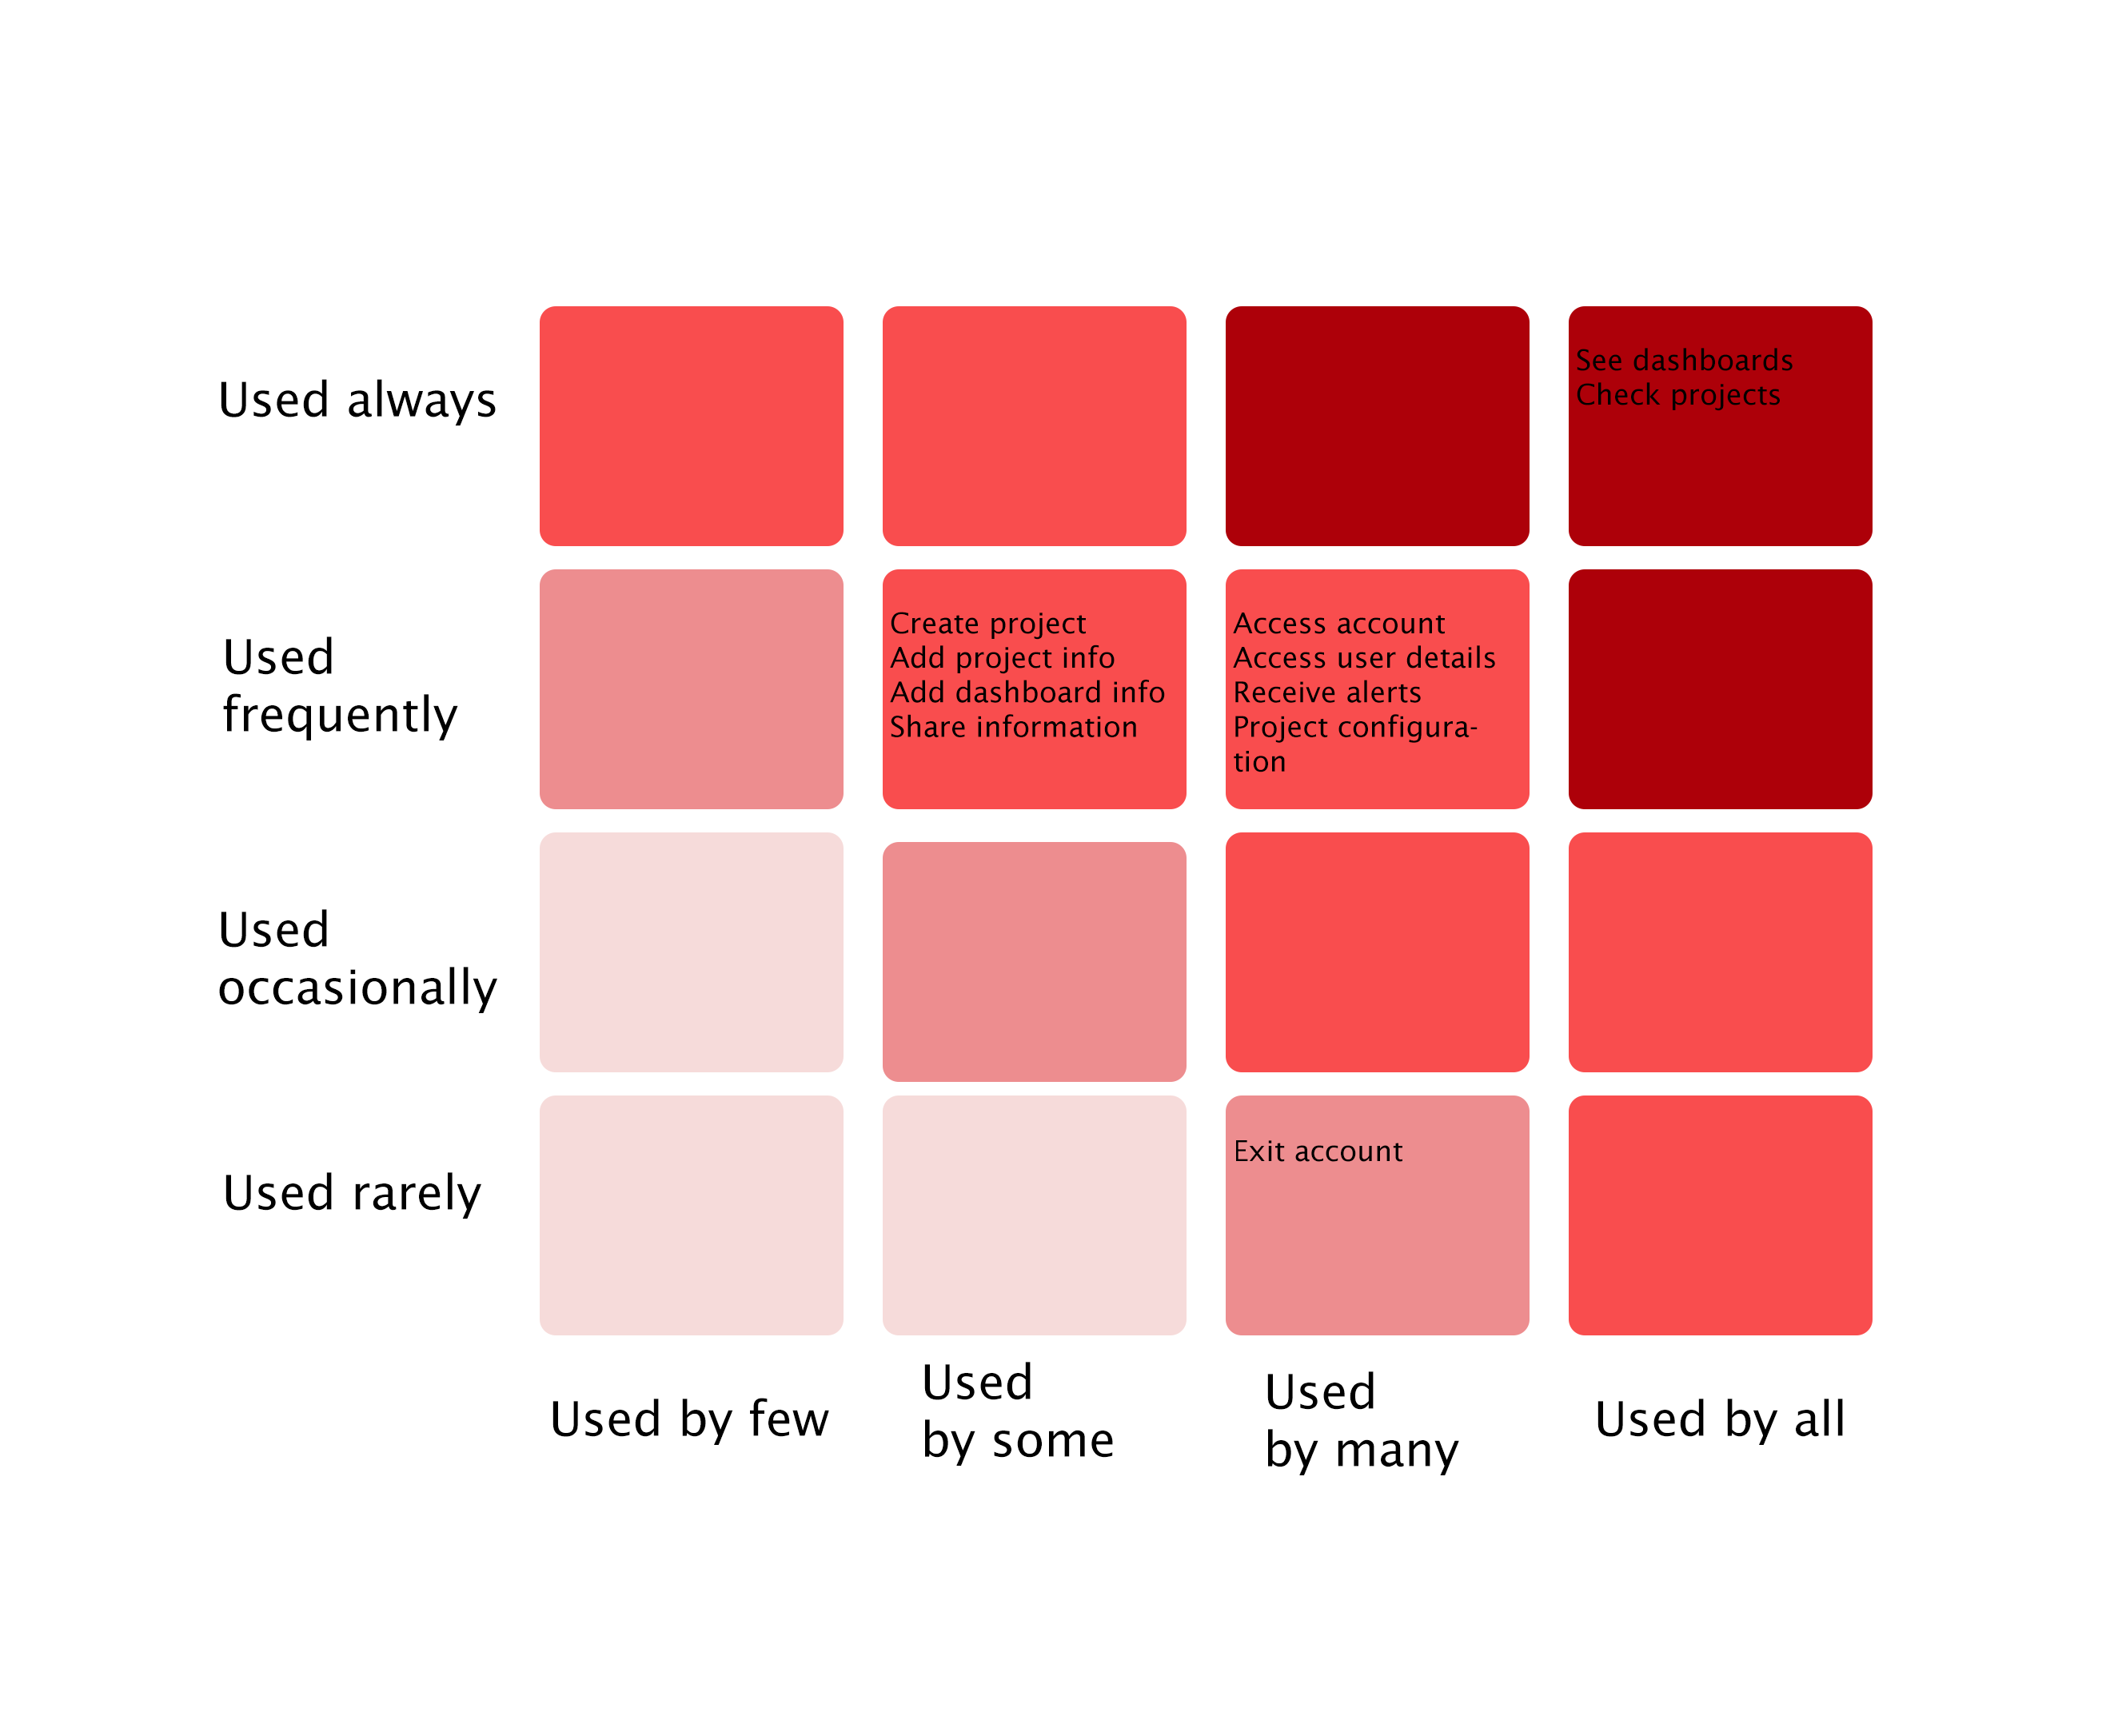
\includegraphics[width=\textwidth]{red-routes.png}
\caption{Red Routes Diagram}
\end{figure}

The team designed the Red Routes for Lean Dashboard application, as we can see in figure 4.1, based on the list of Personas that Inetum provided. We took into account the above factors to create the Red Routes in the best way possible.
\newpage

\section{Information Architecture}
Information architecture(IA) consists of capability of sorting and designing the content of not only the web, but also websites and mobile applications. 
The main purpose of information architecture is to organize content to facilitate the users' process of tuning to the product's functionality and thus, finding anything they might want easily.
There are several elements that can affect the content structure, among which, IA experts tend to regard the specifics of the target audience's needs. This can be justified by the fact that the IA prioritizes user satisfaction.
The main factor that leads people to visit different websites is content. It is commonly shared that producing valuable content for users is crucial, but so is ensuring that the content is easily found. We use Personas that Inetum provided as a tool to find the most adequate IA, and ran usability tests.
 
\begin{figure}[h!]
\center
    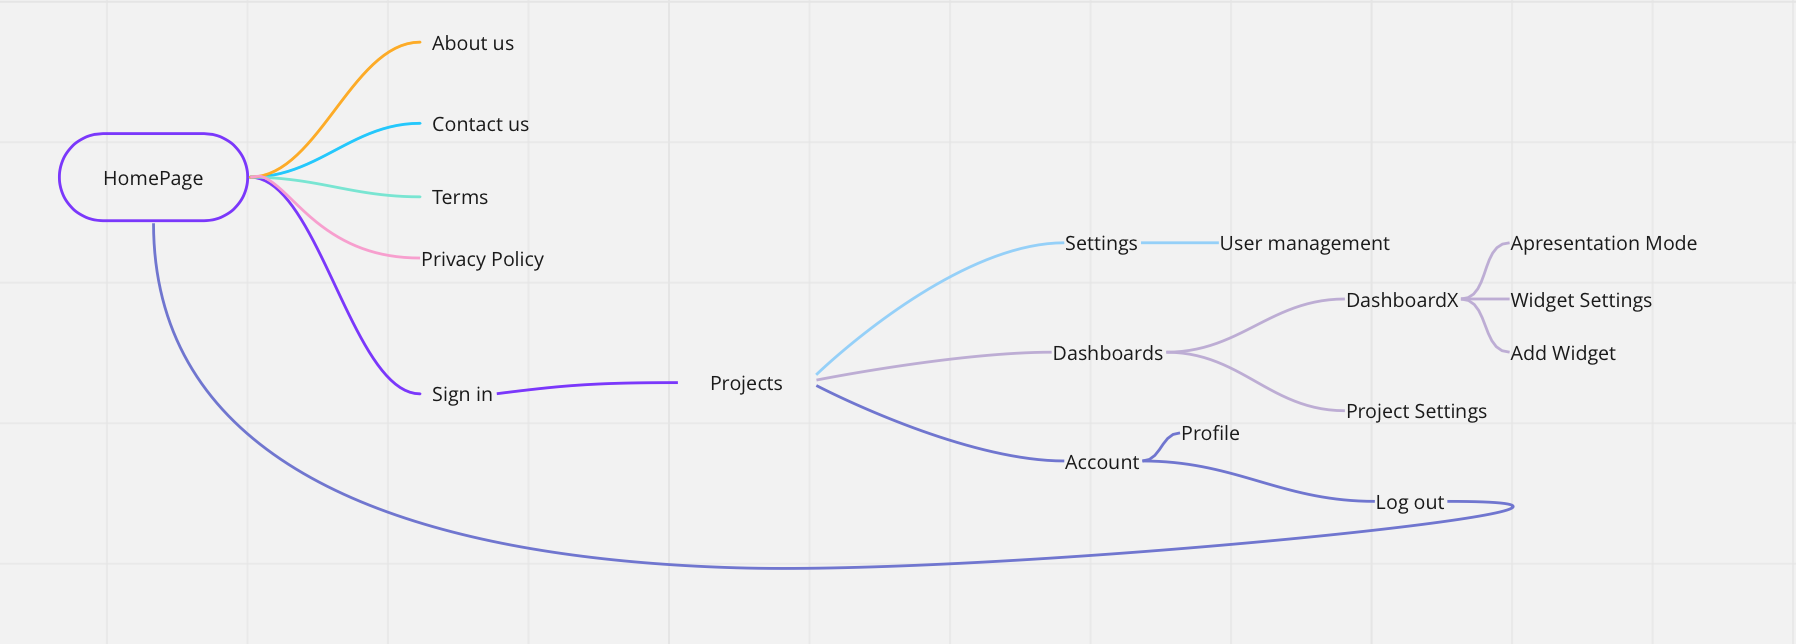
\includegraphics[width=\textwidth]{information-architecture.png}
\caption{Information Architecture Diagram}
\end{figure}

With this diagram, we can better plan the making to the various resources by achieving a flowchart that dictates if the various flowchart accesses make sense (and easily correct them if they don't).

\newpage
\section{Digital Prototype}
A Digital Prototype is a tool used in UX research to develop a mock user interface that can be utilized in use-case tests. These tests gather a small group of people and establish a task that all users need to complete. 
 
A Digital Prototype is how we validate our basic idea and the premises underpinning it by collecting user feedback.
With the obtained results, we can then determine what aspects need to be addressed in the Digital Prototype by us developed.
 
This research and planning done beforehand (before the full implementation of the client application) can greatly decrease implementation costs since it is much easier to make modifications to this mocked user interface than it is to make some of the same changes on the client application code.
We utilized the platform Figma\cite{FIGMA} to develop our Digital Prototype on figure 4.3:
 
\begin{figure}[h!]
\center
    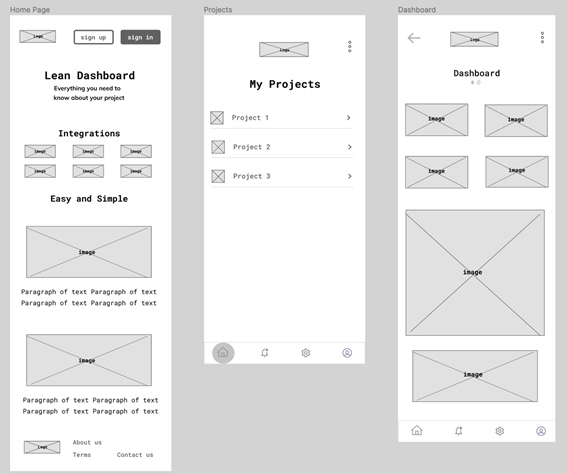
\includegraphics[width=\textwidth]{digital-prototype.png}
\caption{Application Digital Prototype}
\end{figure}

\chapter{Client Application}
The following section explains the current implementation for the client’s side of the application. This section is responsible for the visual of the system.
 
\section{React vs Angular}
React was our choice over Angular. The reason behind such decision was that Angular has a lot of concepts and syntax to learn, as well as the fact that Angular's documentation is much longer and we believe it might take some time to learn a new language given that the time frame is relatively short. React is easier to learn in the short term than Angular and the group that is developing this project would attend a course to learn react, which would be an asset.
 
\section{User Interface}
In this project phase, we only implement the HomePage, Sign in and Sign up pages. The reason for that is because we are finishing the usability tests that can have an impact on our pages and for that reason, we are waiting for the tests to end to starting implement the rest of the pages. 
 
\begin{figure}[h!]
\center
    \includegraphics[width=\textwidth]{HomePage.png}
\caption{Home Page}
\end{figure}
\begin{figure}[h!]

In figure 5.1, we have the Home Page, it is the first page the user sees. The page has 6 components. 
In the header, we have buttons for the user to register or login in and enter the application.
In the footer, we have 4 links with information about the team and application such as About, Terms, Privacy Policy and, contact us.

In figure 5.2, is the view that represents the entrance to the user account. It is composed by a form of two text input boxes that receive the username and the password.
\center
    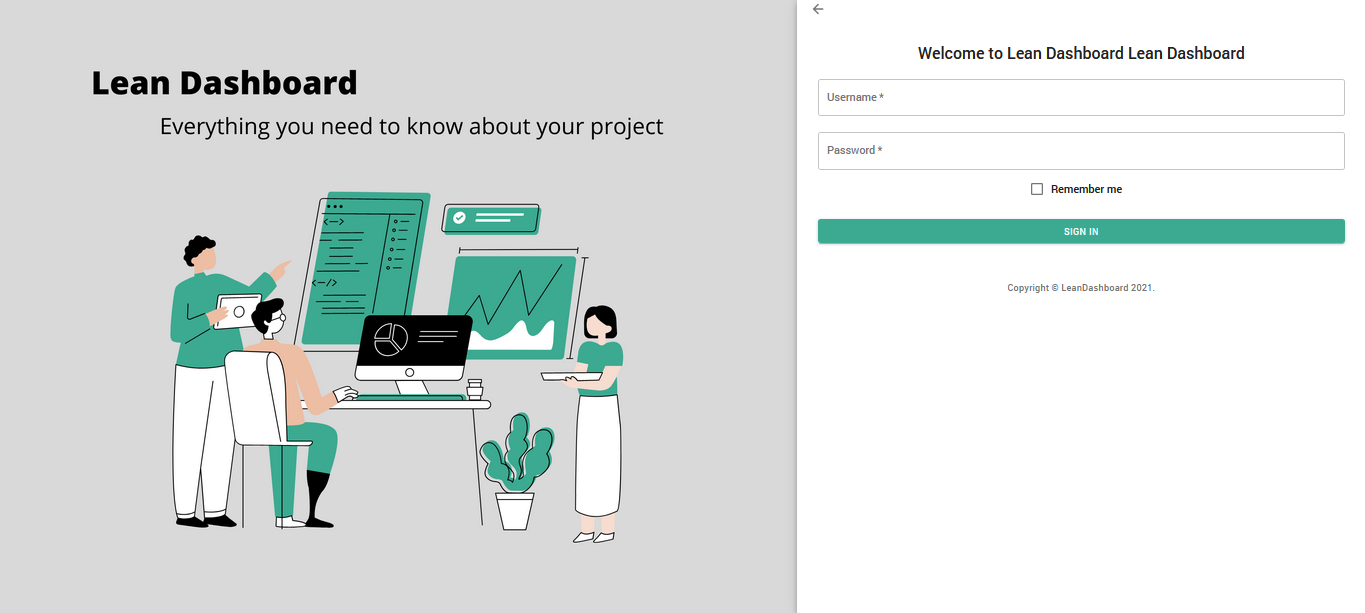
\includegraphics[width=\textwidth]{SignIn.png}
\caption{Sign In}
\end{figure}

\chapter{Conclusion}

Developing this project, allowed the team to apply the experience acquired along the course in this project.

This project provided the opportunity to work with Inetum and developing a web application, from back to front, as well as interacting with other applications in order
to learn how to implement the necessary API requests to obtain the ETL data.

The project also taught the group a lot about the research and planning of an application's user experience as the team has never been introduced to such a topic. Conducting the research on UX and usability tests showed us a new perspective on application development.

According to our initial planning, some of the tasks took longer than we were expecting, especially the ETL procedure as it took some time to learn and adapt to our application, but overall the application is taking shape since as of the date of this report the only core part missing is the single page application and its interaction with the Web API, though some parts are already implemented like the Home Page and the Login Page.





\begin{thebibliography} {websites}

\bibitem{INETUM} Inetum https://gfi.world/pt-en/

\bibitem{JIRA} Jira- Software development tool used by agile teams
https://www.atlassian.com/software/jira

\bibitem{SQUASH} Squash - Suite tool for test management
https://www.squashtest.com/?lang=en

\bibitem{AZURE} Azure - Cloud computing service by Microsoft
https://azure.microsoft.com/en-us/

\bibitem{RBAC} RBAC - Role-based Access Control
\texttt{https://en.wikipedia.org/wiki/Role-based\_access\_control}

\bibitem{INFOARCH} Information Architecture
\texttt{https://en.wikipedia.org/wiki/Information\_architecture}

\bibitem{REACT} React https://reactjs.org/

\bibitem{ETLPROC} ETL - Understanding It and Effectively Using It.
https://medium.com/hashmapinc/etl-understanding-it-and-effectively-using-it-f827a5b3e54d
Consulted on April 1st 2021

\bibitem{AUTHIZATION} Authization Module
https://github.com/dleandro/Authentication-and-Authorization-Node-Component-

\bibitem{POSTGRESQL} PostgreSQL: The World's Most Advanced Open Source Relational Database
https://www.postgresql.org/

\bibitem{MIRO} Miro - Platform used for the Information Architecture schema
https://miro.com/

\bibitem{FIGMA} Figma Prototype toolhttps://www.figma.com/prototyping/

\bibitem{ES} ElasticSearch  https://www.elastic.co/elasticsearch/

\bibitem{NODE} Node.JS  https://nodejs.org/en/

\bibitem{NODECRON} node-cron  https://www.npmjs.com/package/node-cron
\end{thebibliography}
\end{document}